\input intro
\input circuit
\input program


\section{Amostras - laser vermelho}\label{red}

Distancia da fresta ao objeto = \SI{872,0 \pm 1e0}{cm}
Largura do laser no objeto = \SI{11,35 \pm 5e-2}{mm}

\end{multicols}

\begin{center}
\begin{enumerate}

	\item Verificação da colheira do sinal na fenda dupla.

\input red/dupla_red

	\item Colheita do sinal na fenda dupla - houve uma leve falha no inicio devido à localização do  sensor em frente ao sinal da difração

\input red/simples_red_pissed



\end{enumerate}
\end{center}

\begin{multicols}{2}    % 2 columns

\section{Amostras - laser verde}\label{green}

\end{multicols}
\begin{enumerate}

\item Fenda simples, laser verde

\vspace{2cm}
\begin{center}
\begin{tikzpicture}[scale=1.5]
%	\draw[very thin,color=gray] (-0.1,-0.1) grid (9*0.7+0.9,8*0.7+0.9);

	\draw[->] (-0.2,0) -- (9*0.7+1,0) node[below left] {$x$};
	\draw[->] (0,-0.2) -- (0,8*0.7+1) node[right] {$f(x)$};

	\tikz \draw plot[smooth] file {./simples.table};
\end{tikzpicture}
\vspace{1.5cm}
\\\hypertarget{diagrama}{Dados capturados - Fenda Simples}
\end{center}

\item Fenda dupla, laser verde

\vspace{1.5cm}
\begin{center}
\begin{tikzpicture}[scale=1.5]
%	\draw[very thin,color=gray] (-0.1,-0.1) grid (9*0.7+0.9,8*0.7+0.9);

	\draw[->] (-0.2,0) -- (9*0.7+1,0) node[below left] {$x$};
	\draw[->] (0,-0.2) -- (0,8*0.7+1) node[right] {$f(x)$};

	\tikz \draw plot[smooth] file {./dupla.table};
\end{tikzpicture}
%\vspace{0.2cm}
\\\hypertarget{diagrama}{Dados capturados - Fenda Dupla}
\end{center}
	
\end{enumerate}
\begin{multicols}{2}    % 2 columns
